\subsection*{Problema 14}

\textbf{Enunciado:} Calcular la integral:
\begin{align*}
\int \dfrac{x^5 + 2}{x^2 - 1} \, dx
\end{align*}

\textbf{Solución:} Dado que el grado del numerador ($5$) es mayor que el grado del denominador ($2$), realizamos la división polinómica de $x^5 + 2$ entre $x^2 - 1$. 

Dividiendo $x^5$ entre $x^2$, obtenemos $x^3$. Multiplicando y restando, continuamos el proceso hasta obtener el cociente y el residuo indicado:
\begin{align*}
\dfrac{x^5 + 2}{x^2 - 1} = x^3 + x + \dfrac{x + 2}{x^2 - 1}
\end{align*}

Sustituimos esta expresión en la integral original:
\begin{align*}
\int \dfrac{x^5 + 2}{x^2 - 1} \, dx = &\int \left( x^3 + x + \dfrac{x + 2}{x^2 - 1} \right) dx \\
= &\int x^3 \, dx + \int x \, dx \\
&+ \int \dfrac{x + 2}{x^2 - 1} \, dx
\end{align*}

Para la tercera integral, descomponemos el integrando en fracciones parciales:
\begin{align*}
\dfrac{x + 2}{x^2 - 1} = \dfrac{x + 2}{(x-1)(x+1)} = \dfrac{A}{x-1} + \dfrac{B}{x+1}
\end{align*}

Resolviendo para los coeficientes $A$ y $B$, encontramos que $A = \frac{3}{2}$ y $B = -\frac{1}{2}$. Por lo tanto:
\begin{align*}
\dfrac{x + 2}{x^2 - 1} = \dfrac{3}{2(x-1)} - \dfrac{1}{2(x+1)}
\end{align*}

Integramos cada término por separado:
\begin{align*}
\int x^3 \, dx &= \dfrac{x^4}{4} \\
\int x \, dx &= \dfrac{x^2}{2} \\
\int \dfrac{\frac{3}{2}}{x-1} \, dx &= \dfrac{3}{2} \ln|x-1| \\
\int \dfrac{-\frac{1}{2}}{x+1} \, dx &= -\dfrac{1}{2} \ln|x+1|
\end{align*}

Agrupando todos los resultados y añadiendo la constante de integración $C$, obtenemos la solución general:
\begin{align*}
F(x) = &\dfrac{x^4}{4} + \dfrac{x^2}{2} + \dfrac{3}{2} \ln|x-1| \\
&- \dfrac{1}{2} \ln|x+1| + C
\end{align*}

\begin{figure}[H]
	\centering
	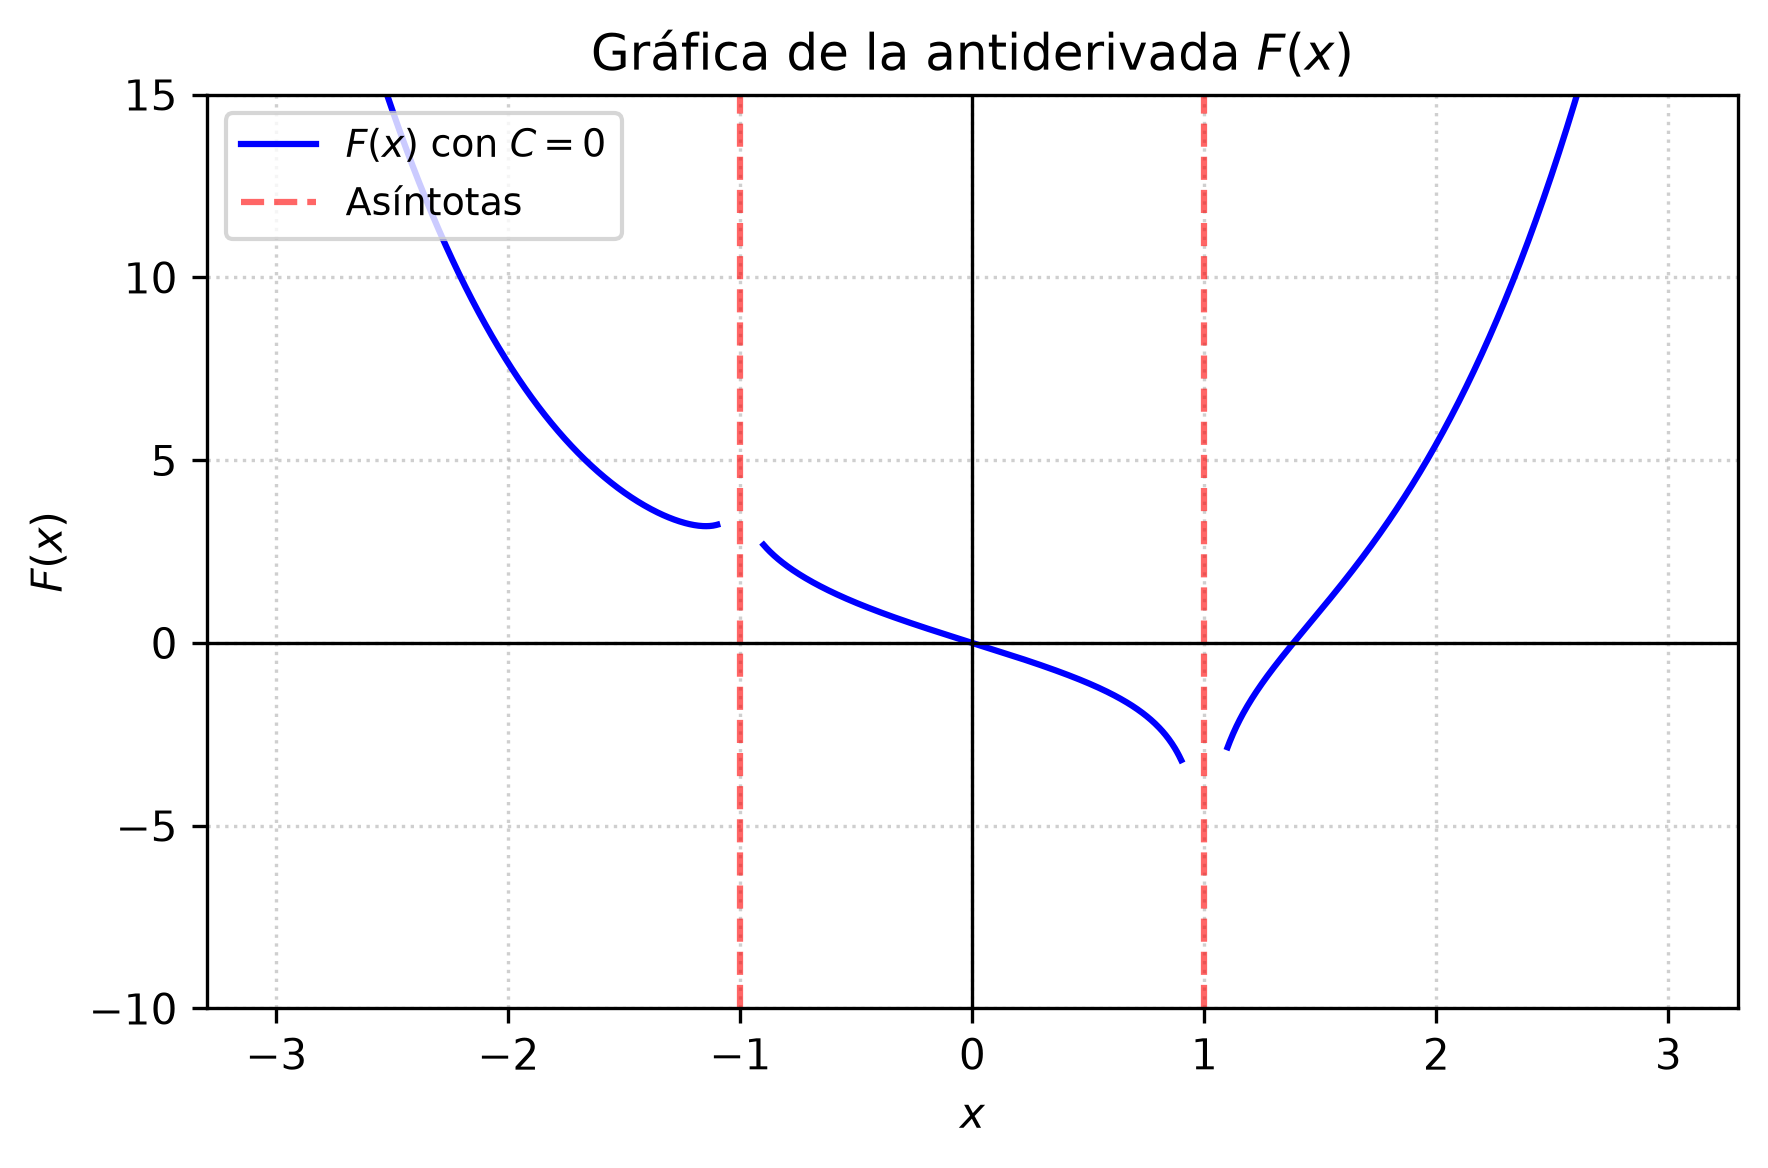
\includegraphics[width=\columnwidth]{semana_03/graficas/SEM03_P14_grafica.png}
	\caption{Representación gráfica de $f(x)$ y su antiderivada $F(x)$ evaluada para la constante de integración $C = 0$ (Problema 14).}
	\label{fig:problema14}
\end{figure}
